\documentclass[../final_report.tex]{subfiles}
\usepackage{subfiles}
\usepackage{diagbox}
\graphicspath{{../../Lab5/plots/}}
\begin{document}

Αντικείμενο μελέτης της συγκεκριμένης άσκησης ήταν η εκτέλεση του αλγορίθμου K-means σε αρχιτεκτονική GPU.
Μελετάμε διαφορετικές τεχνικές με τις οποίες μπορούμε να δομήσουμε ένα πρόγραμμα που θα εκτελεστεί σε GPU και πως
μπορούμε να αξιοποιήσουμε όλο το υλικό για να μειώσουμε τον χρόνο εκτέλεσης, κρατώντας την GPU συνεχώς busy.

% \subsubsection*{Σύντομη Παρουσίαση Υλικού - Αναφορά στο μοντέλο εκτέλεσης SIMT}

% Τρέχοντας query μέσω του NVIDIA System Management Interface (nvidia - smi), αναγνωρίζουμε ότι η κάρτα γραφικών που
% χρησιμοποιούμε για να τρέξουμε τα προγράμματα είναι η NVIDIA Tesla K40c.

\subsection{Τεχνικές υλοποίησης αλγορίθμων που εκτελούνται σε αρχιτεκτονικές GPU}

Στον προγραμματισμό με χρήση επιταχυντών, ο κλασσικός επεξεργαστής συνεχίζει να εκτελεί σημαντικό έργο, αρχικοποιώντας
και μεταφέροντας δεδομένα.

Ο χρόνος σειριακής εκτέλεσης:

\begin{itemize}
    \item \{Size, Coords, Clusters, Loops\} = \{256, 2, 16, 10\} είναι ίσος με 18446.2ms
    \item \{Size, Coords, Clusters, Loops\} = \{256, 16, 16, 10\} είναι ίσος με 5484.8ms
\end{itemize}

\textbf{Σημείωση:} Όλος ο κώδικας της άσκησης βρίσκεται σε ξεχωριστό .zip αρχείο στο Helios της ομάδας.


\subsection{K-Means Naive}
Η πρώτη υλοποίηση είναι και η πιο απλοϊκή σε σκέψη. Δρομολογούμε όσα νήματα όσα και τα στοιχεία του πίνακα στον οποίο εκτελούμε
τον αλγόριθμο K-means. Κάθε νήμα, με συγκεκριμένο thread ID, βρίσκει την κοντινότερη απόσταση από κάποιο κέντρο καλώντας την συνάρτηση euclid\_dist\_2.
Τέλος, αυξάνουμε το μέγεθος membership του κέντρου αυτού.

Οι διαστάσεις του πίνακα objects, είναι αριθμός\_αντικειμένων x αριθμός\_συντεταγμένων. 

Εφόσον τα warps, δηλαδή οι ομάδες των νημάτων, είναι πολλαπλάσια των 32, κάνουμε έναν έλεγχο ορίων ώστε αν δρομολογηθούν νήματα με 
thread ID μεγαλύτερο από τον αριθμό των αντικειμένων στον πίνακα, να μην δράσουν ώστε να μην επιχειρήσουν να αναζητήσουν στοιχείο σε 
διεύθυνση μνήμης που δεν έχει γίνει allocated.

Μεταξύ κάθε iteration, μεταφέρουμε από την CPU στην GPU τους πίνακες των κέτρων (Clusters) και από την GPU στην CPU τον πίνακα
membership, ώστε να γίνει η ανανέωση των κέτρων των cluster. Η CPU αναλαμβάνει την ανανέωση αυτή.

\subsubsection*{K-Means Naive - Αποτελέσματα}

\begin{figure}[H]
    \centering
    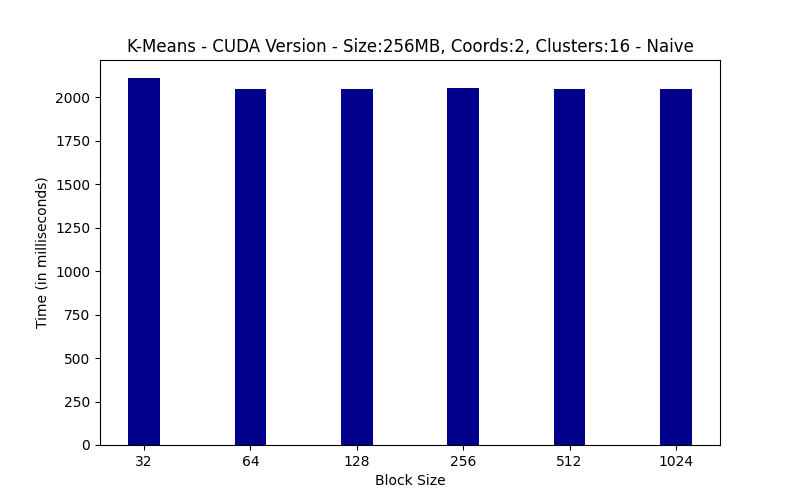
\includegraphics[scale=0.40]{/outFiles/plots/kmeans_gpu_Naive_2_time.png}
    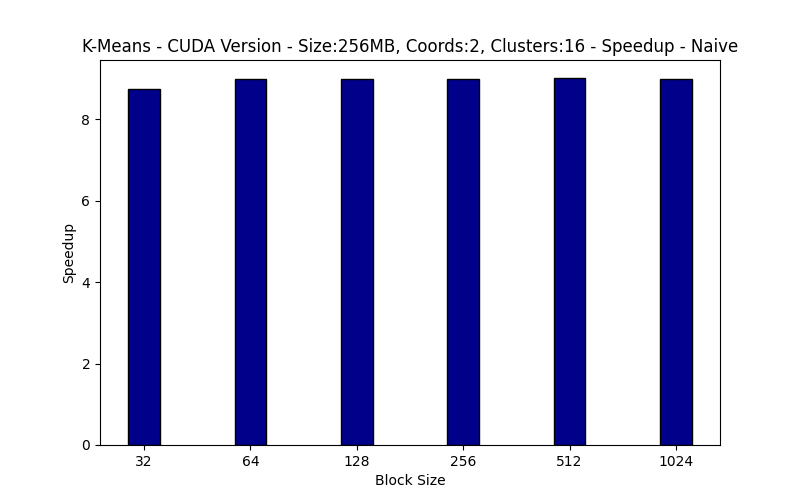
\includegraphics[scale=0.40]{/outFiles/plots/kmeans_gpu_Naive_2_speedup.png}
    \caption{K-Means Naive - GPU Edition}
    \label{fig:K-Means Naive - GPU Edition}
\end{figure}

\subsubsection*{K-Means Naive - Συμπεράσματα}

Η επίδοση της παράλληλης έκδοσης είναι εμφανώς καλύτερη από την σειριακή. Δεδομένου την απλότητα της υλοποίησης, το speedup
είναι αρκετά αξιοσημείωτο. Περαιτέρω, οι παράλληλες εκδόσεις με GPU έχουν το έξτρα overhead της μεταφοράς δεδομένων. Οι μετρήσεις
που κάναμε λαμβάνουν υπόψιν τους το φανόμενο αυτό, ώστε να είναι δίκαιη η σύγκριση με την σειριακή υλοποίηση.

Το block size δεν φαίνεται να επηρεάζει τα αποτελέσματα σε αυτή την υλοποίηση. Με βάση το CUDA Occupancy Calculator, προτιμούμε block size
ίσο με 128 καθώς είναι το πιο ισορροπημένο που δίνει occupancy ίσο με 100\%.

\textbf{Σημείωση:} Ο υπολογισμός του occupancy έγινε με βάση το αρχείο spreadsheet της NVIDIA. Δεν είναι πλήρως ορθό κριτήριο
για την επιλογή του block size. Πιο μοντέρνοι - application specific τρόποι υπολογισμού του occupancy είναι προτιμότερες επιλογές.

\subsubsection*{K-Means Naive - Best Time}

2051.098108ms - 128 Block Size

\subsection{K-Means Transpose}
Το πρώτο βήμα προς την βελτιστοποίηση είναι να ακολουθήσουμε μια πιο architectural aware προσέγγιση. Το προφανές πρόβλημα της naive 
υλοποίησης είναι η κακή πρόσβαση στην μνήμη. Εδώ επιχειρούμε να λύσουμε αυτό το πρόβλημα δίνοντας παραπάνω σημασία στο memory coalescing.
Η υλοποίηση αυτή είναι ίδια με την σημαντική διαφορά ότι αλλάζουμε την λίστα των δεδομένων objects και clusters από row-based
σε column-based indexing. Ανανεώνουμε και την συνάρτηση εύρεσης απόστασης μεταξύ 2 σημείων σε column-based δεικτοδότηση.

\subsubsection*{K-Means Transpose - Αποτελέσματα}

\begin{figure}[H]
    \centering
    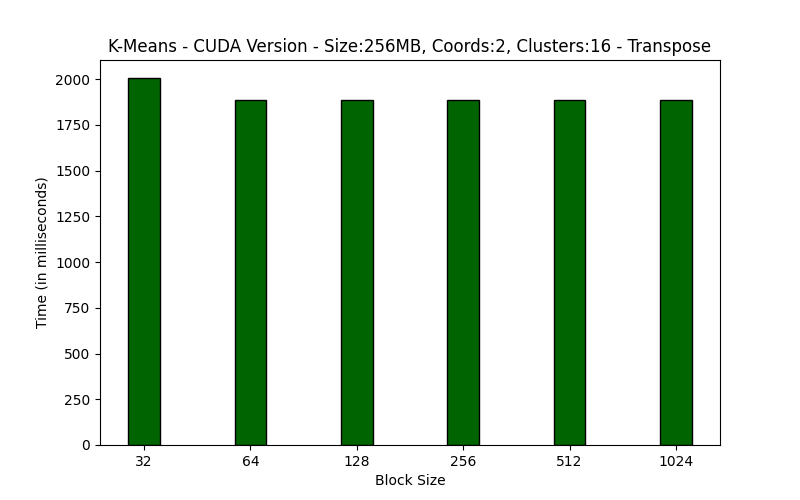
\includegraphics[scale=0.40]{/outFiles/plots/kmeans_gpu_Transpose_2_time.png}
    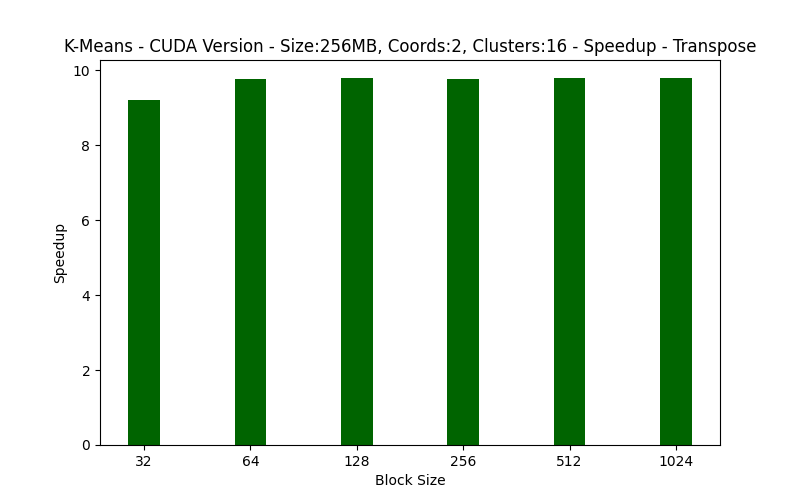
\includegraphics[scale=0.40]{/outFiles/plots/kmeans_gpu_Transpose_2_speedup.png}
    \caption{K-Means Transpose - GPU Edition}
    \label{fig:K-Means Transpose - GPU Edition}
\end{figure}

\subsubsection*{K-Means Transpose - Συμπεράσματα}
Παρατηρούμε αρκετά καλύτερα αποτελέσματα από την Naive έκδοση. Η αλλαγή στην συμπεριφορά του προγράμματος είναι 
αρκετά μικρή αλλά είναι επίσης πιο architectural aware. Στην προηγούμενη έκδοση, η πρόσβαση στην μνήμη ήταν συνεχόμενη αλλά
μη ευθυγραμμισμένη. Για μια δεδομένη σειρά νημάτων που έκανε πρόσβαση στον πίνακα Clusters (με διαστάσεις x:numClusters, y:numCoords),
η πρώτη θέση μνήμης που έκανε πρόσβαση το κάθε νήμα ήταν μια σειρά μακριά. Άρα, γινόντουσαν πολλαπλά memory transactions για να υπολογιστούν
οι αποστάσεις. Το ίδιο πρόβλημα παρουσιαζόταν και στον πίνακα των αντικειμένων (Objects, με διαστάσεις x:numObjs, y:numCoords)

Το πρόβλημα αυτό λύνεται κάνοντας τις προσβάσεις στην μνήμη συνεχόμενες ΚΑΙ ευθυγραμμισμένες. Αυτό πετυχαίνεται κάνοντας transpose τους προαναφερόμενους
πίνακες.

Το block size πάλι δεν φαίνεται να επηρεάζει σημαντικά τα αποτελέσματα. Με εξαίρεση το blockSize=32, οι υπόλοιπες επιλογές παρουσιάζουν
πρακτικά ολόιδια αποτελέσματα. Επιλέγουμε ως βέλτιστο το blockSize=128, για τον ίδιο λόγο που εξηγήσαμε και στην Naive έκδοση (occupancy).

% Κάνε σχήματα να το δείξεις κιολας βλακάκο

\subsubsection*{K-Means Transpose - Best Time}
1883.369207ms - 128 Block Size

\subsection{K-Means Shared Memory}
Το τελευταίο άμεσο βήμα βελτιστοποίησης είναι να εκμεταλευτούμε παραπάνω το ίδιο το υλικό. Οι \textbf{Streaming Multiprocessors} της κάρτας
γραφικών περιέχουν shared memory. Η ειδική αυτή μνήμη, δίνει την δυνατότητα στα νήματα ίδιων block να προσπελαύνουν δεδομένα πιο γρήγορα. Στην υλοποίηση αυτή, τοποθετούμε
τον πίνακα cluster, δηλαδή τον πίνακα που περιέχει τις συντεταγμένες των κέντρων των cluster, στην διαμοιραζόμενη μνήμη. Η υπόλοιπη υλοποίηση
είναι ολόιδια με την Transpose.

\subsubsection*{K-Means Shared Memory - Αποτελέσματα}

\begin{figure}[H]
    \centering
    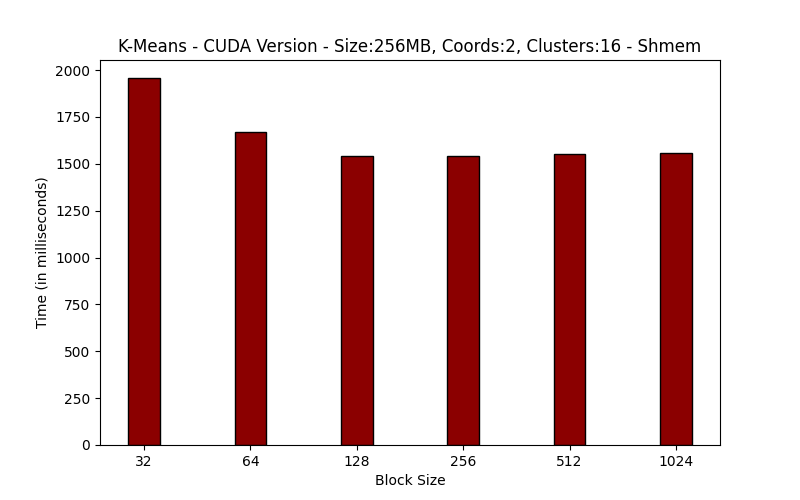
\includegraphics[scale=0.40]{/outFiles/plots/kmeans_gpu_Shmem_2_time.png}
    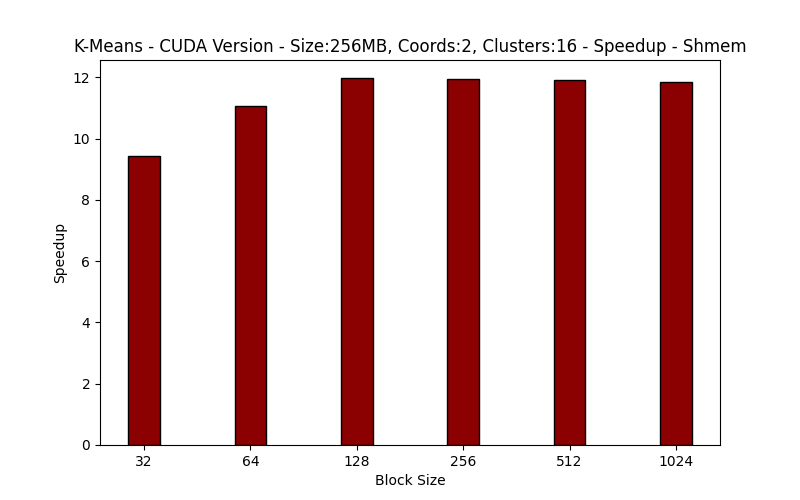
\includegraphics[scale=0.40]{/outFiles/plots/kmeans_gpu_Shmem_2_speedup.png}
    \caption{K-Means Shared - GPU Edition}
    \label{fig:K-Means Shared - GPU Edition}
\end{figure}

\subsubsection*{K-Means Shared Memory - Συμπεράσματα}
Τα αποτελέσματα είναι τα βέλτιστα συγκριτικά με τις 3 υλοποιήσεις. Η shared memory είναι μια πιο ελεγχόμενη μορφή μνήμης cache, στην οποία μπορούμε αναλόγως
το πρόβλημα, να τοποθετήσουμε και διαφορετικά δεδομένα, συγκεκριμένα αυτά που χρησιμοποιούνται πιο συχνά. Σημαντικό είναι να τοποθετούμε τα δεδομένα με σωστό τρόπο
ώστε να αποφευχθούν τα bank conflicts.

Η μείωση του χρόνου είναι λογική αφού χρησιμοποιούμε μνήμη πιο πάνω στην ιεραρχία από αυτήν που χρησιμοποιούσαμε στην Transpose/Naive έκδοση. Πλέον, οι προσπελάσεις
γίνονται γρηγορότερα. Η μοιραζόμενη μνήμη είναι κοινή για νήματα που βρίσκονται στο ίδιο block. Με βάση το occupancy calculator, και στα 2 configurations που μελετάμε,
γίνεται υψηλή χρήση των SM.

Το block size συνεχίζει να μην παίζει κάποιο ρόλο στην εκτέλεση του προγράμματος, βέλτιστο είναι πάλι οτιδήποτε πάνω ή ίσο με 128 νήματα.

\subsubsection*{K-Means Shared Memory - Best Time}
1541.312933ms - 128 Block Size

\subsection{Σύγκριση υλοποιήσεων / bottleneck Analysis / μελέτη άλλων configuration}

Από τις 3 υλοποιήσεις, λογικό η καλύτερη να είναι αυτή που αξιοποιεί και την μοιραζόμενη μνήμη αλλά και το memory coalescing, δηλαδή, η Shared Memory version.
Οι χρόνοι εκτέλεσεις και το speedup παρουσιάζονται σε κοινό διάγραμμα και για τις 3 εκδόσεις παρακάτω. 
\begin{figure}[H]
    \centering
    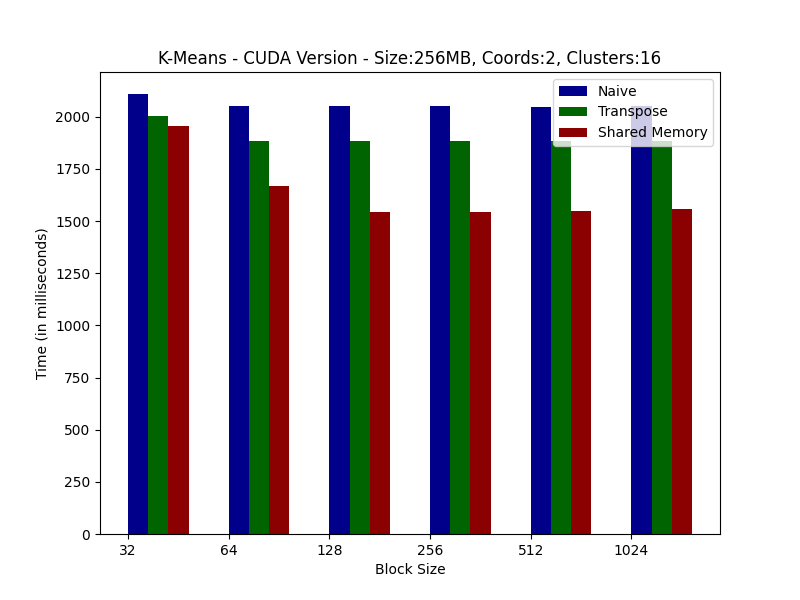
\includegraphics[scale=0.40]{/outFiles/plots/kmeans_gpu_common_figure_2_time.png}
    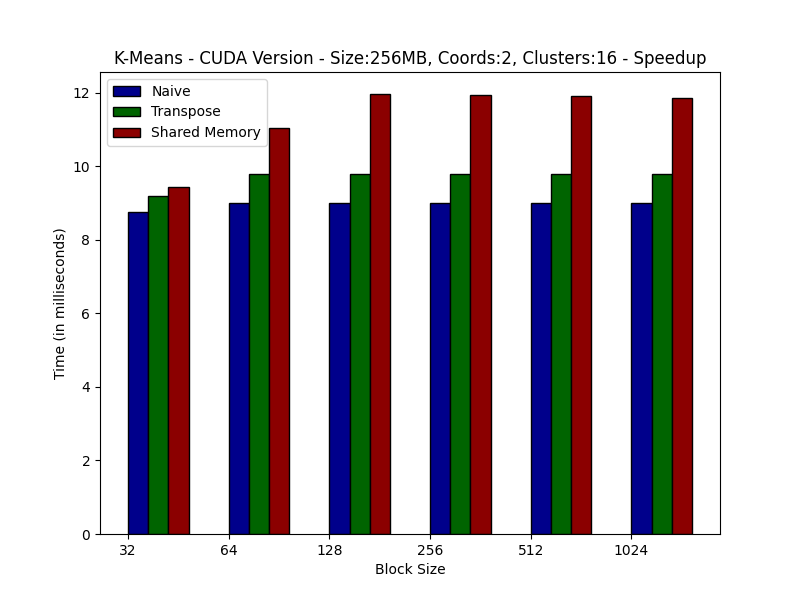
\includegraphics[scale=0.40]{/outFiles/plots/kmeans_gpu_common_figure_2_speedup.png}
    \caption{K-Means - GPU Edition Size - numCoords=2}
    \label{fig:K-Means - GPU Edition - {Size:256Mb, numCoords:2, numClusters:16}}
\end{figure}

\subsubsection*{Bottleneck Analysis}
Προσθέτουμε 3 ξεχωριστά timers (CPU, Transfer, GPU) για να μελετήσουμε πιο μέρος του συστήματος απαιτεί τον
περισσότερο χρόνο. Οι πίνακες είναι κατά μέσο όρο για όλα τα block sizes που μελετάμε και σε millisecond.

\noindent
\begin{tabular}{|l||*{4}{c|}}\hline
\backslashbox{Type}{Timers}
&\makebox[5em]{CPU Timer}&\makebox[6.5em]{Transfer Timer}&\makebox[5em]{GPU Timer}
\\\hline\hline
Naive & 887.971 & 406.153 & 765.745\\\hline
Transpose & 797.969 & 406.419 & 701.031\\\hline
Shared Memory & 796.91 & 406.115 & 433.498\\\hline

\end{tabular}

\hfill

Το μέγεθος της μεταφοράς των δεδομένων είναι ίδιο και για τις 3 υλοποιήσεις και δεν μπορούμε να επέμβουμε
για να βελτιωθεί με κάποιον τρόπο. Είναι αναγκαίο κακό του προγραμματισμού ετερογενών συστημάτων.

Διαδοχικά, μειώνεται ο χρόνος εκτέλεσης του μέρους που εκτελείται από την GPU καθώς βελτιώνονται οι υλοποιήσεις.

Το μέρος που εκτελείται στον επεξεργαστή είναι περίπου σταθερό, παρατηρούμε όμως μια μικρή μείωση, κοντά στα 10\%,
μεταξύ της Naive έκδοσης και των Transpose/Shared Memory. Αυτή δικαιολογείται γιατί πλέον ο υπολογισμός των νέων κέντρων
γίνεται με βάση τον transposed πίνακα, που είναι ελάχιστα πιο cache-friendly (τουλάχιστον για το συγκεκριμένο configuration).

Το κυριότερο bottleneck είναι η εκτέλεση στον CPU και η μεταφορά των δεδομένων. Ο συνολικός χρόνος εκτέλεσης μπορεί να 
μειωθεί περαιτέρω αν μεταφερθεί όλη η εκτέλεση του αλγορίθμου στην GPU. Έτσι, περιορίζεται δραστικά η συνεχόμενη μεταφορά 
δεδομένων μεταξύ host και device. Επίσης, αξιοποιούμε το γεγονός ότι μπορεί, έστω στοιχειωδώς, να παραλληλοποιηθεί το task 
εύρεσης νέων κέντρων.

\begin{figure}[H]
    \centering
    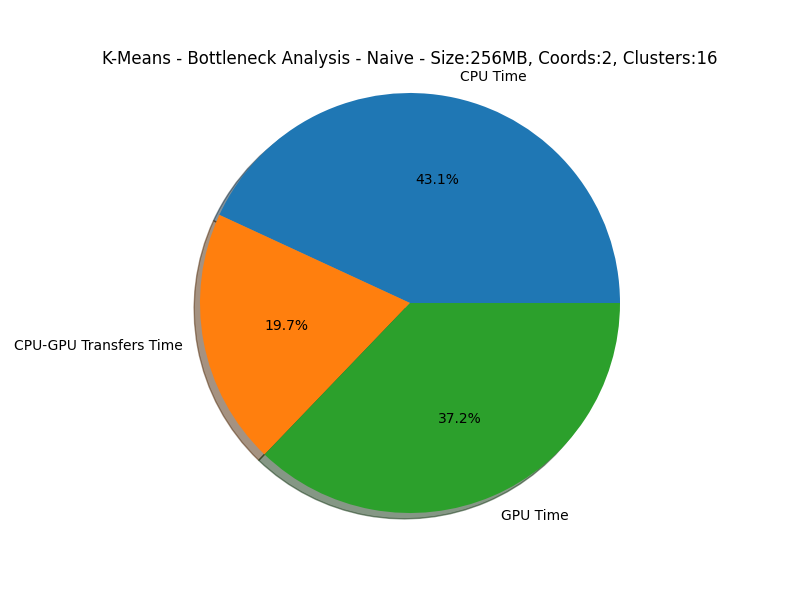
\includegraphics[scale=0.40]{/outFiles/plots/kmeans_gpu_Naive_2_bottleneck_analysis.png}
    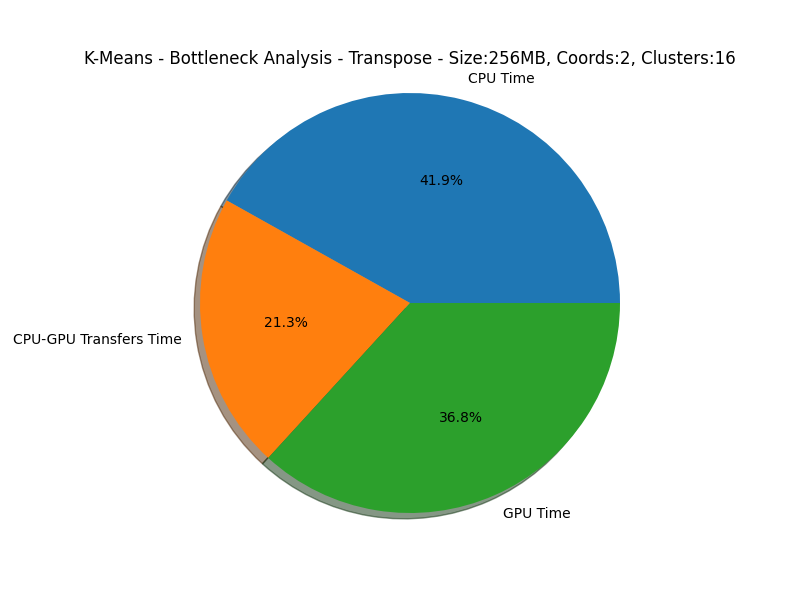
\includegraphics[scale=0.40]{/outFiles/plots/kmeans_gpu_Transpose_2_bottleneck_analysis.png}
    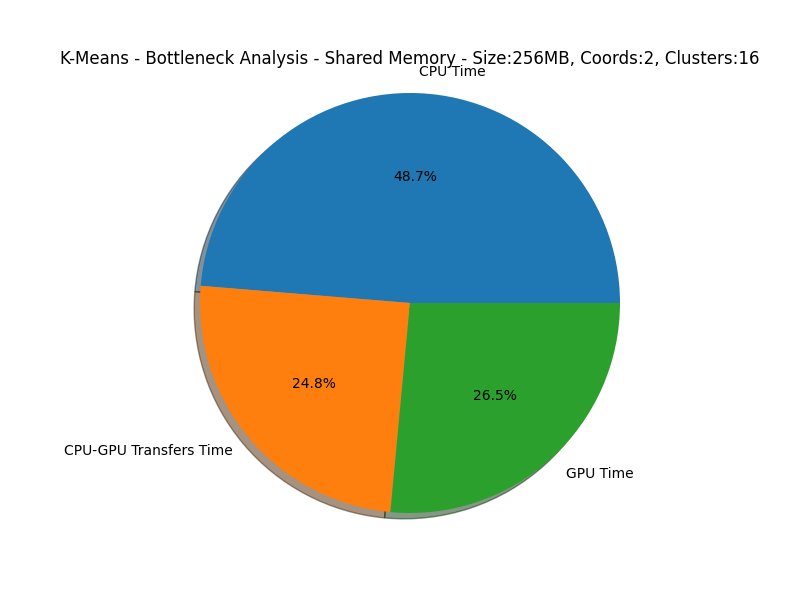
\includegraphics[scale=0.40]{/outFiles/plots/kmeans_gpu_Shmem_2_bottleneck_analysis.png}
    \caption{K-Means - Bottleneck Analysis - numCoords=2}
    \label{fig:K-Means - Bottleneck Analysis - numCoords=2}
\end{figure}

\subsubsection*{Μελέτη Άλλων Configuration}

Δημιουργούμε τα γραφήματα των ίδιων υλοποιήσεων για το configuration \{Size, Coords, Clusters, Loops\} = \{256, 16, 16, 10\}.
Τα "σφάλματα" στην σχεδίαση του Naive αλγορίμου είναι πιο ξεκάθαρα εδώ. Το γεγονός ότι δεν εκμεταλέυεται την ικανότητα των 
GPU για memory coalescing και, αντιθέτως, απαιτούνται πολλαπλά transactions για τον υπολογισμό των αποστάσεων, περιορίζει πολύ την
επίδοσή της. 

Η transpose έκδοση είναι πάνω από 5 φορές καλύτερη στο GPU μέρος αλλά 2 φορές χειρότερη στο CPU μέρος. Η χειροτέρευση 
του CPU μέρους εξηγείται από το γεγονός ότι υπολογίζουμε τα νέα κέντρα με column-based δεικτοδότηση η οποία δεν είναι τόσο 
cache-friendly (τουλάχιστον στο συγκεκριμένο configuration).

Το κόστος της μεταφοράς είναι πάλι κοινό για όλες τις μεταφορές. Η shared έκδοση μπορεί να βελτιωθεί στο κομμάτι που αναλαμβάνει η CPU.
Μια καλή λύση θα ήταν να ξαναγίνεται transpose ο πίνακας πριν μεταφερθεί στην CPU, καθώς η GPU μπορεί να κάνει αυτό το transpose πολύ πιο σύντομα.



\begin{figure}[H]
    \centering
    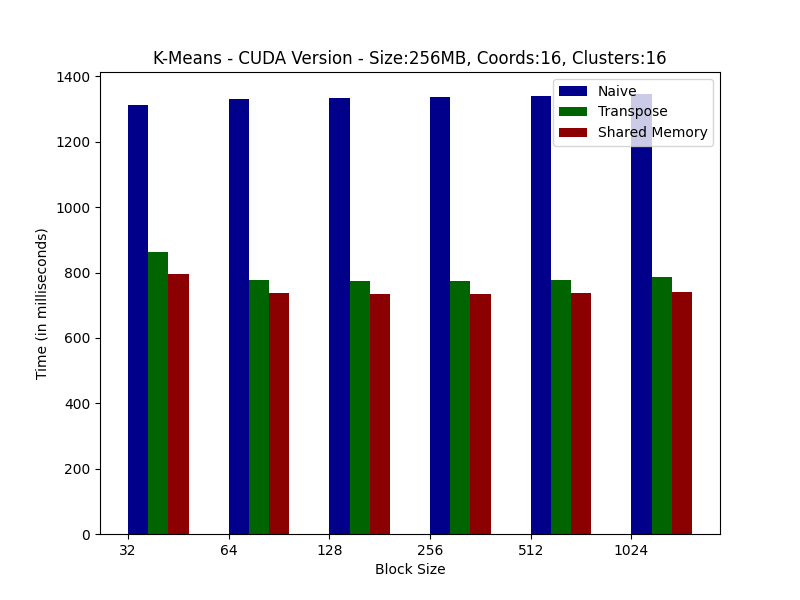
\includegraphics[scale=0.38]{/outFiles/plots/kmeans_gpu_common_figure_16_time.png}
    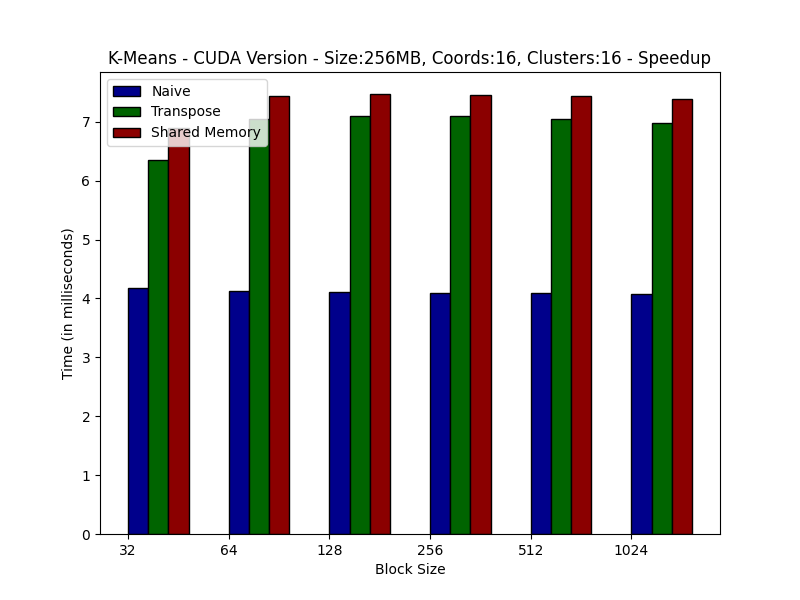
\includegraphics[scale=0.38]{/outFiles/plots/kmeans_gpu_common_figure_16_speedup.png}
    \caption{K-Means - GPU Edition Size - numCoords=16}
    \label{fig:K-Means - GPU Edition - {Size:256Mb, numCoords:16, numClusters:16}}
\end{figure}

\noindent
\begin{tabular}{|l||*{4}{c|}}\hline
\backslashbox{Type}{Timers}
&\makebox[5em]{CPU Timer}&\makebox[6.5em]{Transfer Timer}&\makebox[5em]{GPU Timer}
\\\hline\hline
Naive & 214.842 & 53.018 & 1065.877\\\hline
Transpose & 550.324 & 53.009 & 188.571\\\hline
Shared Memory & 549.727 & 53.006 & 144.105\\\hline
\end{tabular}

\begin{figure}[H]
    \centering
    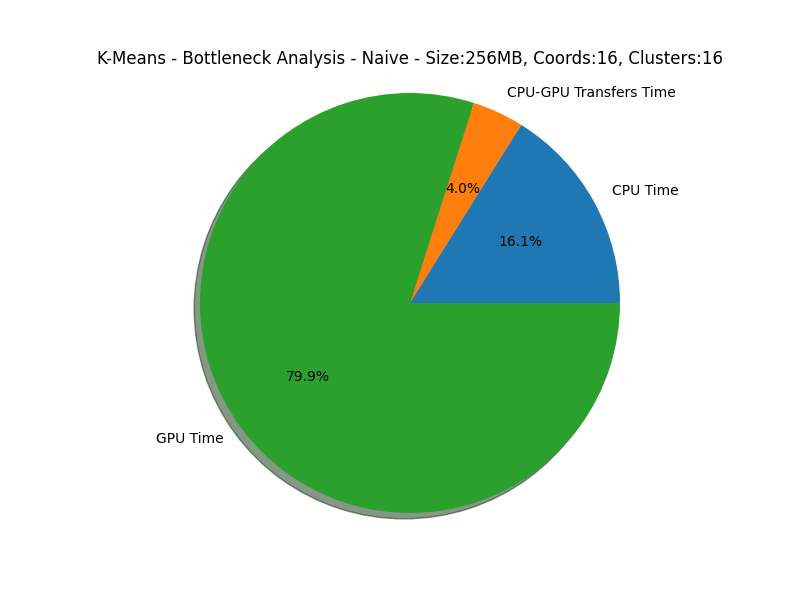
\includegraphics[scale=0.38]{/outFiles/plots/kmeans_gpu_Naive_16_bottleneck_analysis.png}
    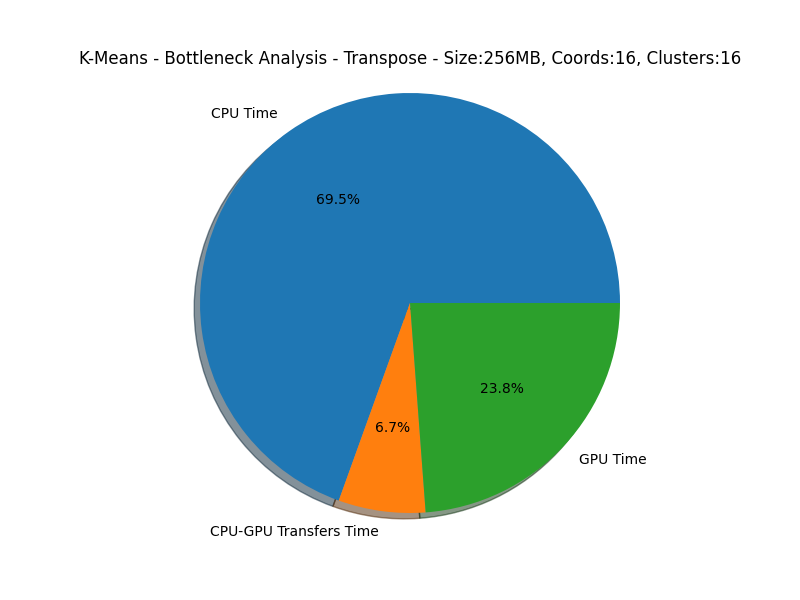
\includegraphics[scale=0.38]{/outFiles/plots/kmeans_gpu_Transpose_16_bottleneck_analysis.png}
    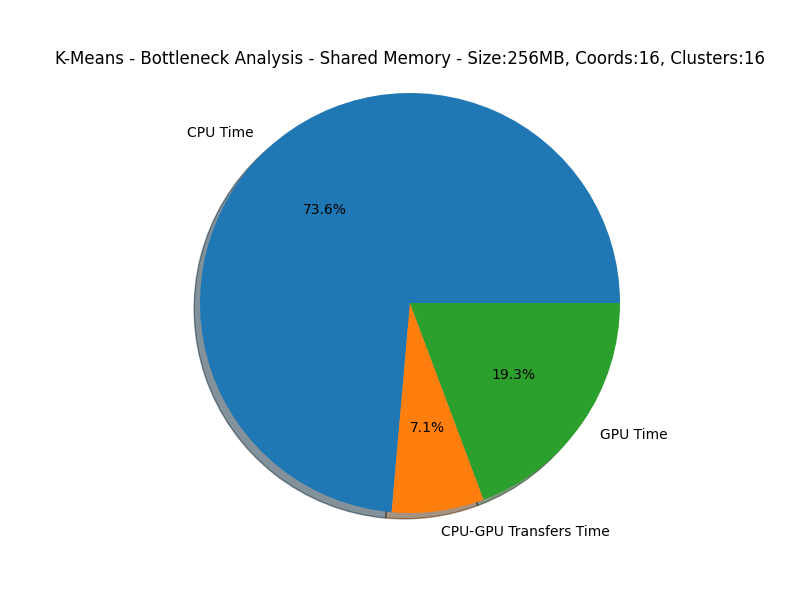
\includegraphics[scale=0.38]{/outFiles/plots/kmeans_gpu_Shmem_16_bottleneck_analysis.png}
    \caption{K-Means - Bottleneck Analysis - numCoords=16}
    \label{fig:K-Means - Bottleneck Analysis - numCoords=16}
\end{figure}

\subsection{K-Means All GPU}
Ακόμα work in progress...

\end{document}